% Provenance (never printed): cycle 2 "Questionner l'espace et le temps ---
% se situer dans l'espace": representations of familiar spaces (plans), "lire
% des plans, se reperer sur des cartes. Elements constitutifs d'une carte :
% titre, echelle, orientation, legende"; see sources/book1/PROVENANCE.md.
% Book 1, grade 2, chapter 2. Sync 1: "scale" is owned here; "cardinal
% directions" is the physics series' term (prose only); "compass rose" here.
\chapter{चित्र से मानचित्र तक}\label{ch:g2:drawing-to-map}

एक कबूतर स्कूल के ऊपर से उड़ रहा है। उसे क्या दिखता है? सामने के दरवाज़े
नहीं, खिड़कियाँ नहीं, बच्चों के चेहरे नहीं: वहाँ ऊपर से उसे चीज़ों का
सिर्फ़ ऊपरी हिस्सा दिखता है। इमारतों की छतें धूसर आयत हैं। आँगन एक बड़ी
ख़ाली आकृति है जिसमें पेड़ों के कुछ गोल शिखर हैं। रास्ते पतली रेखाएँ हैं।
कबूतर स्कूल को ऊपर से देखता है --- वैसे ही जैसे \omterm{def:g2:drawing-to-map:map}{मानचित्र} उसे दिखाता है।

\begin{omfigure}
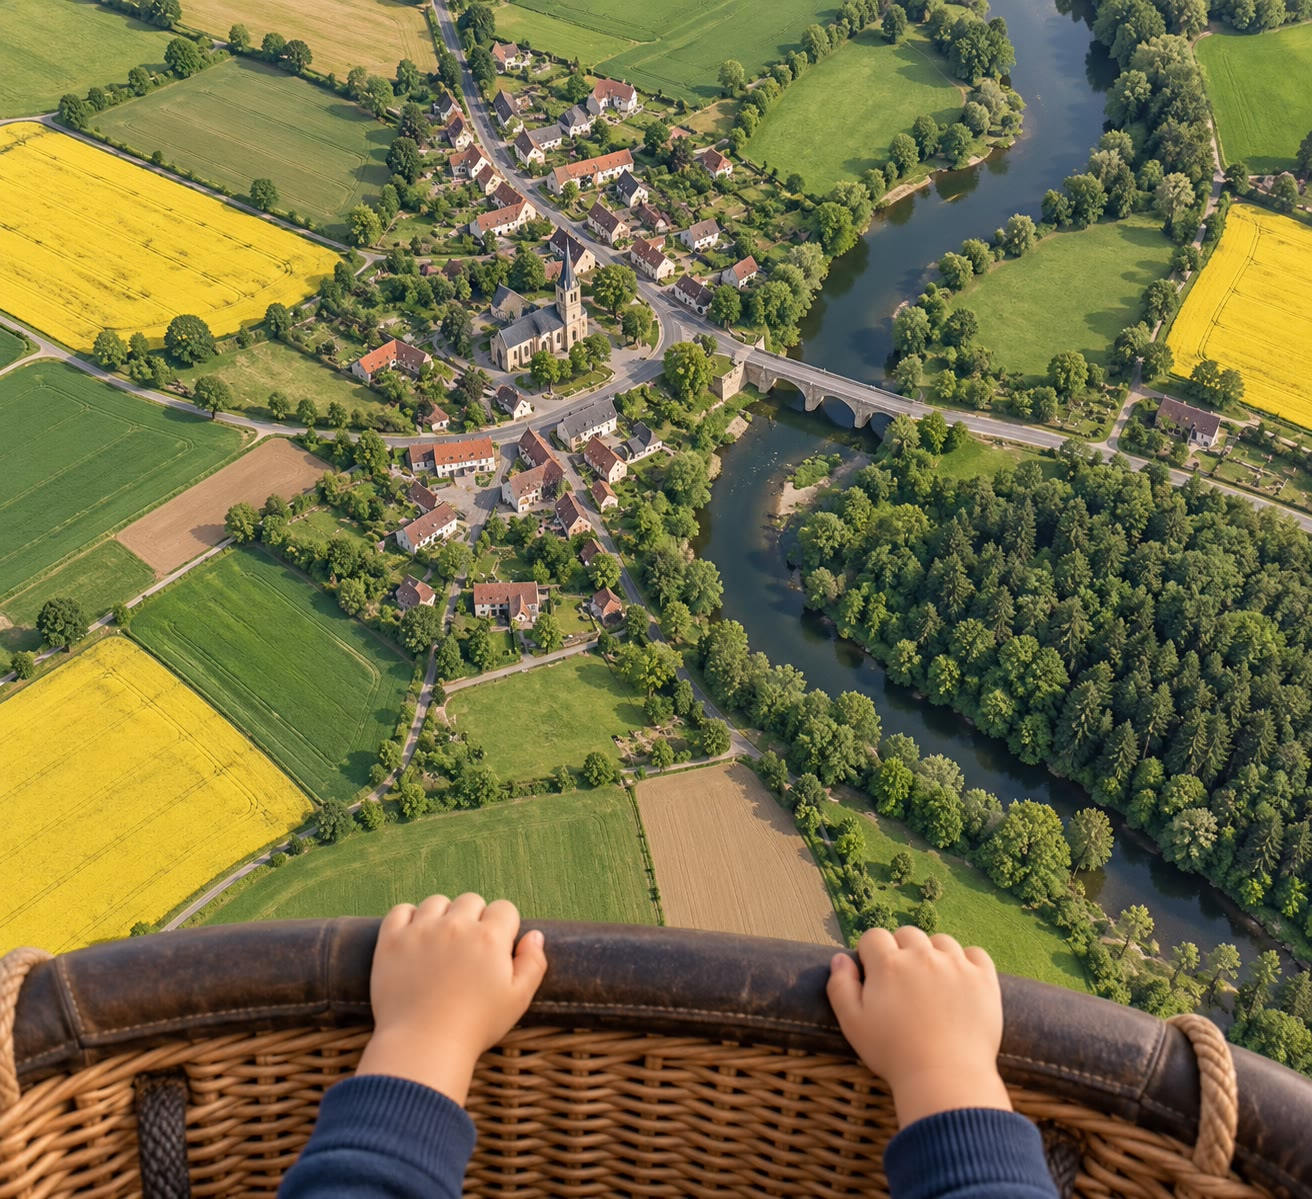
\includegraphics[width=0.62\linewidth]{images/book1/ai/g2-balloon-view.jpg}

{\small गरम हवा के गुब्बारे से दिखता देहात: खेत, एक गाँव, एक सड़क, एक \omterm{def:g1:landscapes-around-us:water}{नदी}
और उसका पुल, सब कुछ ऊपर से देखा हुआ।}
\end{omfigure}

\section{बगल से देखना, ऊपर से देखना}

मेज़ पर खिलौनों के कुछ गुटके रखो। उन्हें बगल से देखो: तुम्हें उनकी
ऊँचाई दिखती है, और पीछे वाले गुटके आगे वालों के पीछे छिप जाते हैं। अब
खड़े होकर उन्हें ऊपर से नीचे की ओर देखो: अब तुम्हें यह नहीं दिखता कि वे
कितने ऊँचे हैं, पर यह ठीक-ठीक दिखता है कि हर गुटका कहाँ है और वे एक-दूसरे
से कितनी दूर हैं।

\begin{omfigure}
\begin{tikzpicture}[x=1cm, y=1cm, font=\small]
  % side view
  \begin{scope}
    \draw[black!50] (-0.2,0) -- (4.6,0);
    \fill[red!55, draw=black!60] (0.2,0) rectangle (1.2,1.6);
    \fill[ocBlue!55, draw=black!60] (1.6,0) rectangle (3.0,0.8);
    \fill[yellow!70, draw=black!60] (3.4,0) -- (3.9,1.1) -- (4.4,0) -- cycle;
    \node at (2.2,-0.5) {बगल से देखा हुआ};
  \end{scope}
  % from above
  \begin{scope}[shift={(6.4,0)}]
    \draw[black!30, fill=black!3] (-0.2,-0.1) rectangle (4.6,2.3);
    \fill[red!55, draw=black!60] (0.2,0.4) rectangle (1.2,1.4);
    \fill[ocBlue!55, draw=black!60] (1.6,1.0) rectangle (3.0,2.0);
    \fill[yellow!70, draw=black!60] (3.9,0.75) circle (0.5);
    \node at (2.2,-0.5) {ऊपर से देखा हुआ};
  \end{scope}
\end{tikzpicture}

{\small मेज़ पर तीन गुटके: एक ऊँचा लाल गुटका, एक चपटा नीला गुटका और एक
पीला शंकु। ऊपर से शंकु एक वृत्त है और ऊँचा गुटका एक वर्ग।}
\label{fig:g2:drawing-to-map:blocks}
\end{omfigure}

\begin{definition}[खाका]\label{def:g2:drawing-to-map:plan}
\emph{खाका}\index{खाका} किसी छोटी जगह --- एक कमरे, एक घर, एक स्कूल,
एक बग़ीचे --- का ऐसा चित्र है जो उसे ठीक ऊपर से देखे हुए रूप में दिखाता
है; वह असल से छोटा बनाया जाता है, पर उसका हर हिस्सा अपनी सही जगह पर होता है।
\end{definition}

\section{छोटा बनाना: मापनी}

कक्षा इतनी बड़ी है कि उसे जैसी है वैसी काग़ज़ के एक पन्ने पर नहीं बनाया जा
सकता। हम उसे छोटा बनाते हैं --- पर हर हिस्से को एक ही तरह से छोटा करना
होगा, नहीं तो \omterm{def:g2:drawing-to-map:plan}{खाका} झूठ बोलेगा। सबसे आसान तरीक़ा है वर्गांकित काग़ज़: काग़ज़
का एक वर्ग कक्षा के एक मीटर के बराबर माना जाता है।

\begin{definition}[मापनी]\label{def:g2:drawing-to-map:scale}
किसी \omterm{def:g2:drawing-to-map:plan}{खाके} या \omterm{def:g2:drawing-to-map:map}{मानचित्र} की \emph{मापनी}\index{मापनी} बताती है कि चित्र असली
जगह से कितना छोटा है: चित्र पर की कोई लंबाई ज़मीन पर कितनी दूरी के
बराबर है। उदाहरण के लिए: \emph{1 वर्ग = 1 मीटर}।
\end{definition}

\begin{omfigure}
\begin{tikzpicture}[x=0.75cm, y=0.75cm, font=\scriptsize]
  \draw[black!15] (0,0) grid (10,8);
  \draw[black, line width=1.6pt] (0,0) rectangle (10,8);
  % board on the north wall
  \fill[black!70] (3,7.8) rectangle (7,8);
  % teacher's desk
  \fill[brown!50, draw=black!70] (4,6) rectangle (6,7);
  % pupils' desks: 3 rows of 3
  \foreach \x in {1,4,7} \foreach \y in {1,2.5,4}
    \fill[orange!45, draw=black!70] (\x,\y) rectangle ++(2,1);
  % cupboard
  \fill[ocBlue!40, draw=black!70] (9,5) rectangle (10,8);
  % door (gap) on the east wall, windows on the west wall
  \fill[white] (9.85,1) rectangle (10.15,2);
  \draw[black!70] (10,2) arc[start angle=90, end angle=180, radius=1];
  \foreach \y in {1.5,4.5}
    \draw[ocBlue, line width=2.5pt] (0,\y) -- (0,\y+2);
  % legend
  \begin{scope}[shift={(11,7.2)}]
    \node[anchor=west, font=\small\bfseries] at (0,0.4) {कक्षा};
    \fill[black!70] (0,-0.25) rectangle (0.8,-0.05); \node[anchor=west] at (1,-0.15) {श्यामपट};
    \fill[brown!50, draw=black!70] (0,-1.1) rectangle (0.8,-0.7); \node[anchor=west] at (1,-0.9) {शिक्षक की मेज़};
    \fill[orange!45, draw=black!70] (0,-1.85) rectangle (0.8,-1.45); \node[anchor=west] at (1,-1.65) {विद्यार्थी की मेज़};
    \fill[ocBlue!40, draw=black!70] (0,-2.6) rectangle (0.8,-2.2); \node[anchor=west] at (1,-2.4) {अलमारी};
    \draw[ocBlue, line width=2.5pt] (0,-3.15) -- (0.8,-3.15); \node[anchor=west] at (1,-3.15) {खिड़की};
    \draw[black!70] (0.8,-3.95) arc[start angle=0, end angle=90, radius=0.6]; \draw[black, line width=1.6pt] (0.2,-3.95) -- (0.8,-3.95); \node[anchor=west] at (1,-3.7) {दरवाज़ा};
    \draw[black!15] (0,-4.9) rectangle (0.75,-4.15);
    \node[anchor=west] at (1,-4.53) {1 वर्ग = 1 मीटर};
    \pic[scale=0.7, transform shape] at (0.7,-6.2) {compassrose};
  \end{scope}
\end{tikzpicture}

{\small वर्गांकित काग़ज़ पर एक कक्षा का \omterm{def:g2:drawing-to-map:plan}{खाका}, अपने शीर्षक, अपनी \omterm{def:g2:drawing-to-map:legend}{संकेत-सूची},
अपनी \omterm{def:g2:drawing-to-map:scale}{मापनी} और अपने \omterm{def:g2:drawing-to-map:directions}{दिशा-चक्र} के साथ। उत्तर की दीवार, जिस पर श्यामपट है,
सबसे ऊपर है।}
\label{fig:g2:drawing-to-map:classroom}
\end{omfigure}
% (exercise data: an invented classroom of 10 m by 8 m)

\begin{method}[खाके पर नापना]\label{met:g2:drawing-to-map:measure}
वर्गों पर बने \omterm{def:g2:drawing-to-map:plan}{खाके} से कोई असली लंबाई जानने के लिए:
\begin{enumerate}
  \item जो लंबाई चाहिए, उसके साथ-साथ वर्ग गिनो;
  \item \omterm{def:g2:drawing-to-map:scale}{मापनी} पढ़ो: एक वर्ग कितने के बराबर है;
  \item जवाब मीटर में दो (या \omterm{def:g2:drawing-to-map:map}{मानचित्र} पर किलोमीटर में)।
\end{enumerate}
\end{method}

\begin{example}[कक्षा कितनी लंबी है?]\label{ex:g2:drawing-to-map:length}
\omterm{def:g2:drawing-to-map:plan}{खाके} में उत्तर की दीवार के साथ-साथ 10 वर्ग हैं। एक वर्ग 1 मीटर के बराबर
है, इसलिए कक्षा 10 मीटर लंबी है। पश्चिम की दीवार के साथ-साथ 8 वर्ग हैं:
वह 8 मीटर चौड़ी है। श्यामपट उत्तर की दीवार के 4 वर्ग घेरता है: वह 4 मीटर
लंबा है।
\end{example}

\begin{omfigure}
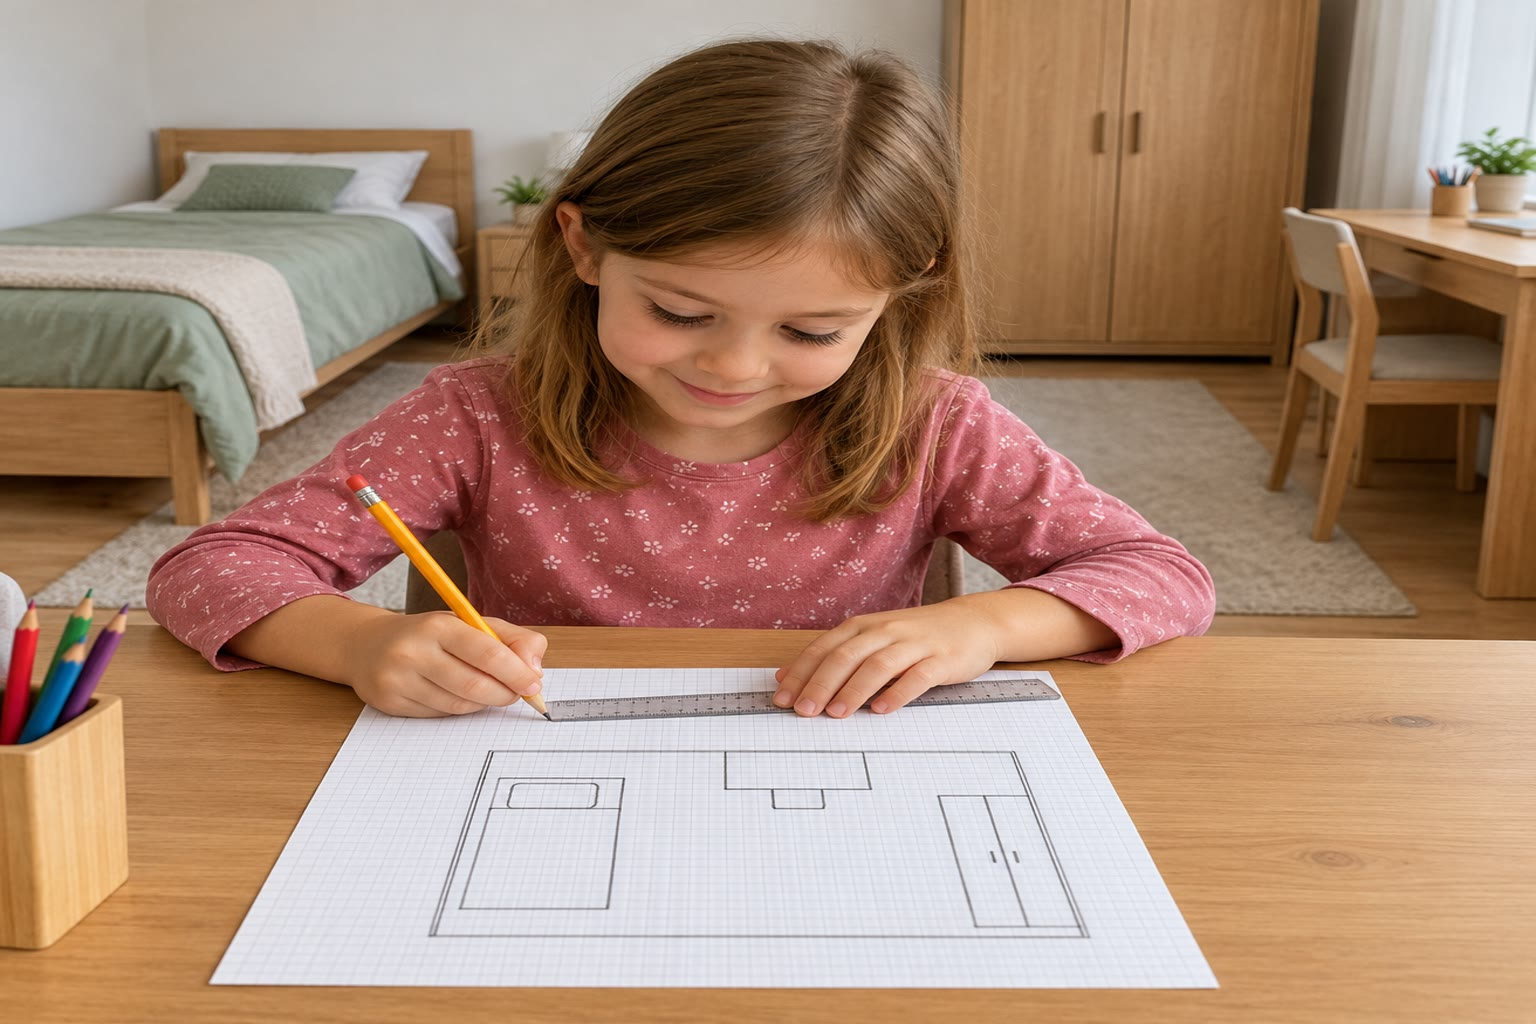
\includegraphics[width=0.55\linewidth]{images/book1/ai/g2-bedroom-plan.jpg}

{\small वर्गांकित काग़ज़ पर सोने के कमरे का \omterm{def:g2:drawing-to-map:plan}{खाका} बनाना।}
\end{omfigure}

\section{खाके से मानचित्र तक}

\omterm{def:g2:drawing-to-map:plan}{खाका} एक छोटी जगह दिखाता है। जब हम कोई बड़ी जगह बनाते हैं --- पूरा शहर, एक
\omterm{def:g1:landscapes-around-us:landform}{घाटी}, एक देश --- तो हम \omterm{def:g2:drawing-to-map:map}{मानचित्र} बनाते हैं।

\begin{definition}[मानचित्र]\label{def:g2:drawing-to-map:map}
\emph{मानचित्र}\index{मानचित्र} पृथ्वी की सतह के किसी बड़े हिस्से का चित्र
है, जो ऊपर से देखा हुआ हो और असल से बहुत छोटा बनाया गया हो।
\end{definition}

\omterm{def:g2:drawing-to-map:map}{मानचित्र} पर एक घर इतना छोटा होता है कि उसे असली रूप में नहीं बनाया जा
सकता, इसलिए \omterm{def:g2:drawing-to-map:map}{मानचित्र} बनाने वाले छोटे-छोटे संकेत इस्तेमाल करते हैं: फ़ार्म
के लिए एक बिंदु, \omterm{def:g1:landscapes-around-us:water}{नदी} के लिए एक नीली रेखा, जंगल के लिए एक हरी आकृति। हर
संकेत का अर्थ \omterm{def:g2:drawing-to-map:map}{मानचित्र} के बगल में एक ख़ाने में दिया होता है।

\begin{definition}[संकेत-सूची]\label{def:g2:drawing-to-map:legend}
\emph{मानचित्र-चिह्न}\index{मानचित्र-चिह्न} एक छोटा संकेत है जो \omterm{def:g2:drawing-to-map:plan}{खाके} या
\omterm{def:g2:drawing-to-map:map}{मानचित्र} पर किसी एक तरह की चीज़ को दिखाता है। \emph{संकेत-सूची}\index{संकेत-सूची}
वह ख़ाना है जिसमें \omterm{def:g2:drawing-to-map:map}{मानचित्र} का हर चिह्न अपने अर्थ के साथ दिखाया जाता है।
\end{definition}

\section{रास्ता ढूँढना: चार दिशाएँ और दिशा-चक्र}

कोई चीज़ कहाँ है, यह बताने के लिए ``बाईं ओर'' या ``दाईं ओर'' कहना काफ़ी
नहीं है: जो तुम्हारी बाईं ओर है, वह तुम्हारे सामने मुँह करके खड़े व्यक्ति
की दाईं ओर है। लोग चार ऐसी दिशाएँ इस्तेमाल करते हैं जो सबके लिए एक जैसी
हैं: उत्तर, पूर्व, दक्षिण और पश्चिम। तुम भौतिकी की पुस्तकों में दिक्सूचक
के साथ इनसे मिल चुके हो। सुबह सूर्य पूर्व में उगता है, और शाम को पश्चिम
में डूबता है; उत्तर और दक्षिण इन दोनों के बीचोंबीच हैं, एक-दूसरे के आमने-सामने।

\begin{omfigure}
\begin{tikzpicture}[font=\small]
  \pic[scale=1.5, transform shape] at (0,0) {compassrose};
  \node[align=left, anchor=west, font=\small] at (2.6,0.3)
    {उ = उत्तर (ज़्यादातर मानचित्रों में सबसे ऊपर)\\पू = पूर्व (दाईं ओर)\\द = दक्षिण (सबसे नीचे)\\प = पश्चिम (बाईं ओर)};
\end{tikzpicture}

{\small एक \omterm{def:g2:drawing-to-map:directions}{दिशा-चक्र}। उत्तर और पूर्व के बीच उत्तर-पूर्व है; दक्षिण और
पश्चिम के बीच, दक्षिण-पश्चिम।}
\label{fig:g2:drawing-to-map:rose}
\end{omfigure}

\begin{definition}[दिशा-चक्र]\label{def:g2:drawing-to-map:directions}
\emph{दिशा-चक्र}\index{दिशा-चक्र} \omterm{def:g2:drawing-to-map:map}{मानचित्र} पर बना वह तारा है जो उत्तर,
पूर्व, दक्षिण और पश्चिम दिशाएँ दिखाता है। ज़्यादातर \omterm{def:g2:drawing-to-map:map}{मानचित्रों} पर उत्तर
सबसे ऊपर, पूर्व दाईं ओर, दक्षिण सबसे नीचे और पश्चिम बाईं ओर होता है।
\end{definition}

\begin{safety}
पूर्व या पश्चिम ढूँढने के लिए सूर्य की ओर कभी मत देखो: इससे तुम्हारी आँखों
को हमेशा के लिए चोट पहुँच सकती है। इसकी जगह परछाइयों को देखो, या दिक्सूचक
का इस्तेमाल करो।
\end{safety}

\section{एक असली मानचित्र पढ़ना}

हर अच्छे \omterm{def:g2:drawing-to-map:map}{मानचित्र} के चार हिस्से होते हैं: एक \textbf{शीर्षक} जो बताता है
कि \omterm{def:g2:drawing-to-map:map}{मानचित्र} क्या दिखाता है, एक \textbf{\omterm{def:g2:drawing-to-map:legend}{संकेत-सूची}}, एक \textbf{\omterm{def:g2:drawing-to-map:scale}{मापनी}}, और
एक \textbf{\omterm{def:g2:drawing-to-map:directions}{दिशा-चक्र}} (या कम से कम उत्तर की ओर इशारा करता एक तीर)। यह रहा
\omterm{def:g1:landscapes-around-us:landform}{पहाड़ियों} वाली एक \omterm{def:g1:landscapes-around-us:landform}{घाटी}, वार्डन पहाड़ियों, का \omterm{def:g2:drawing-to-map:map}{मानचित्र}। यह एक काल्पनिक \omterm{def:g1:landscapes-around-us:landform}{घाटी}
है जिससे तुम इस पुस्तक में और अगली पुस्तकों में बार-बार मिलोगे, हर बार
और ज़्यादा बारीकी से बनी हुई।

\begin{omfigure}
\begin{tikzpicture}
\begin{axis}[width=9.6cm, scale only axis,
    xmin=0, xmax=10, ymin=0, ymax=8, axis equal image,
    xtick={0,...,10}, ytick={0,...,8}, xticklabels={}, yticklabels={},
    grid=major, grid style={black!20}, major tick length=0pt,
    axis background/.style={fill=green!12!omLithAlluv},
    title={\textbf{वार्डन पहाड़ियाँ}}]
  \addplot[fill=omHypsLandD, draw=omHypsLandE!80!black, line width=0.4pt, fill opacity=0.85,
    unbounded coords=jump, even odd rule] table {figdata/out/grade-2-varden_plan-hills.dat};
  \addplot[fill=green!45!black!55, draw=green!35!black, line width=0.4pt] table {figdata/out/grade-2-varden_plan-wood.dat};
  \addplot[ocBlue!85!black, line width=2.2pt] table {figdata/out/shared-region-river.dat};
  \addplot[red!65!black, line width=1.3pt] table {figdata/out/grade-2-varden_plan-road.dat};
  \fill[black] (axis cs:5.012,3.414) ++(-3pt,-4pt) rectangle ++(6pt,8pt);
  \fill[white] (axis cs:5.012,3.414) ++(-1.6pt,-4pt) rectangle ++(3.2pt,8pt);
  \fill[brown!70!black] (axis cs:2.5,3.5) ++(-3.5pt,-3.5pt) rectangle ++(7pt,7pt);
  \fill[red!70!black] (axis cs:7.5,5.5) ++(-5pt,-3pt) rectangle ++(4pt,4pt);
  \fill[red!70!black] (axis cs:7.5,5.5) ++(1pt,-3pt) rectangle ++(4pt,4pt);
  \fill[red!70!black] (axis cs:7.5,5.5) ++(-2pt,2pt) rectangle ++(4pt,4pt);
\end{axis}
\begin{scope}[shift={(10.2,6.4)}, font=\small]
  \node[anchor=west, font=\small\bfseries] at (-0.1,0.55) {संकेत-सूची};
  \fill[omHypsLandD, draw=omHypsLandE!80!black] (0,-0.2) rectangle (0.7,0.15); \node[anchor=west] at (0.85,0) {पहाड़ियाँ};
  \fill[green!45!black!55] (0,-0.85) rectangle (0.7,-0.5); \node[anchor=west] at (0.85,-0.67) {जंगल};
  \draw[ocBlue!85!black, line width=2.2pt] (0,-1.35) -- (0.7,-1.35); \node[anchor=west] at (0.85,-1.35) {नदी};
  \draw[red!65!black, line width=1.3pt] (0,-2.0) -- (0.7,-2.0); \node[anchor=west] at (0.85,-2.0) {सड़क};
  \fill[black] (0.25,-2.8) rectangle (0.45,-2.5); \fill[white] (0.3,-2.8) rectangle (0.4,-2.5); \node[anchor=west] at (0.85,-2.65) {पुल};
  \fill[brown!70!black] (0.23,-3.45) rectangle (0.47,-3.21); \node[anchor=west] at (0.85,-3.33) {फ़ार्म};
  \foreach \dx/\dy in {0.12/-4.1, 0.33/-4.1, 0.22/-3.92}
    \fill[red!70!black] (\dx,\dy) rectangle ++(0.13,0.13);
  \node[anchor=west] at (0.85,-3.98) {गाँव};
  \draw[black!40] (0,-4.95) rectangle (0.5,-4.45); \node[anchor=west, align=left] at (0.85,-4.7) {1 वर्ग\\= 1 किलोमीटर};
  \pic[scale=0.75, transform shape] at (0.8,-6.5) {compassrose};
\end{scope}
\end{tikzpicture}

{\small वार्डन पहाड़ियों का एक सरल \omterm{def:g2:drawing-to-map:map}{मानचित्र}, अपने शीर्षक, अपनी \omterm{def:g2:drawing-to-map:legend}{संकेत-सूची},
अपनी \omterm{def:g2:drawing-to-map:scale}{मापनी} और अपने \omterm{def:g2:drawing-to-map:directions}{दिशा-चक्र} के साथ। \omterm{def:g1:landscapes-around-us:water}{नदी} पश्चिम से पूर्व की ओर बहती है।}
\label{fig:g2:drawing-to-map:varden}
\end{omfigure}
% (figdata/grade-2/varden_plan.py; the region: figdata/shared/region.py)

\begin{method}[मानचित्र पढ़ना]\label{met:g2:drawing-to-map:read}
\begin{enumerate}
  \item शीर्षक पढ़ो: \omterm{def:g2:drawing-to-map:map}{मानचित्र} कौन-सी जगह दिखाता है?
  \item \omterm{def:g2:drawing-to-map:legend}{संकेत-सूची} पढ़ो: हर चिह्न का क्या अर्थ है?
  \item \omterm{def:g2:drawing-to-map:directions}{दिशा-चक्र} ढूँढो: उत्तर कहाँ है?
  \item \omterm{def:g2:drawing-to-map:scale}{मापनी} पढ़ो, और दूरियाँ जानने के लिए वर्ग गिनो।
\end{enumerate}
\end{method}

\begin{example}[फ़ार्म से गाँव तक]\label{ex:g2:drawing-to-map:farm}
वार्डन पहाड़ियों के \omterm{def:g2:drawing-to-map:map}{मानचित्र} पर फ़ार्म \omterm{def:g1:landscapes-around-us:water}{नदी} के दक्षिण में है। गाँव जाने के
लिए किसान पूर्व की ओर सड़क पकड़ता है, पुल से \omterm{def:g1:landscapes-around-us:water}{नदी} पार करता है, और आगे
उत्तर-पूर्व की ओर चलता है। गाँव फ़ार्म से 5 वर्ग पूर्व में और 2 वर्ग उत्तर
में है: यानी 5 किलोमीटर पूर्व की ओर और 2 किलोमीटर उत्तर की ओर।
\end{example}

\section{अभ्यास}

\begin{exercise}[$\star$]\label{exo:g2:drawing-to-map:1}
\omterm{def:g2:drawing-to-map:plan}{खाका} बगल से देखे हुए रूप में बनाया जाता है, या ऊपर से देखे हुए रूप में?
\end{exercise}

\begin{exercise}[$\star$]\label{exo:g2:drawing-to-map:2}
कक्षा के \omterm{def:g2:drawing-to-map:plan}{खाके} में पश्चिम की दीवार पर नीले रंग से क्या बना है? उत्तर-पूर्वी
कोने में क्या है?
\end{exercise}

\begin{exercise}[$\star$]\label{exo:g2:drawing-to-map:3}
उन चार हिस्सों के नाम बताओ जो हर अच्छे \omterm{def:g2:drawing-to-map:map}{मानचित्र} में होने चाहिए।
\end{exercise}

\begin{exercise}[$\star$]\label{exo:g2:drawing-to-map:4}
ज़्यादातर \omterm{def:g2:drawing-to-map:map}{मानचित्रों} पर सबसे ऊपर कौन-सी दिशा होती है? बाईं ओर कौन-सी?
\end{exercise}

\begin{exercise}[$\star$]\label{exo:g2:drawing-to-map:5}
कक्षा के \omterm{def:g2:drawing-to-map:plan}{खाके} में विद्यार्थी की एक मेज़ 2 वर्ग गुणा 1 वर्ग जगह घेरती है।
असली कक्षा में मेज़ कितनी लंबी और कितनी चौड़ी है?
\end{exercise}

\begin{exercise}[$\star$]\label{exo:g2:drawing-to-map:6}
वार्डन पहाड़ियों के \omterm{def:g2:drawing-to-map:map}{मानचित्र} पर भूरा वर्ग किस चीज़ के लिए है? और हरी
आकृति?
\end{exercise}

\begin{exercise}[$\star\star$]\label{exo:g2:drawing-to-map:7}
वार्डन पहाड़ियों के \omterm{def:g2:drawing-to-map:map}{मानचित्र} पर जंगल \omterm{def:g1:landscapes-around-us:water}{नदी} के उत्तर में है या दक्षिण में?
वह फ़ार्म के पूर्व में है या पश्चिम में?
\end{exercise}

\begin{exercise}[$\star\star$]\label{exo:g2:drawing-to-map:8}
वार्डन पहाड़ियों का पूरा \omterm{def:g2:drawing-to-map:map}{मानचित्र} पश्चिम से पूर्व तक 10 वर्ग और दक्षिण से
उत्तर तक 8 वर्ग का है। हर दिशा में यह कितने किलोमीटर हुआ?
\end{exercise}

\begin{exercise}[$\star\star$]\label{exo:g2:drawing-to-map:9}
कक्षा के \omterm{def:g2:drawing-to-map:plan}{खाके} में विद्यार्थियों की कितनी मेज़ें हैं? एक विद्यार्थी दरवाज़े
के सबसे पास वाली मेज़ पर बैठता है। वह मेज़ कक्षा के उत्तर में है या दक्षिण में?
\end{exercise}

\begin{exercise}[$\star\star$]\label{exo:g2:drawing-to-map:10}
लूकस अपने सोने के कमरे का \omterm{def:g2:drawing-to-map:plan}{खाका} बनाता है। उसका पलंग 2 मीटर लंबा है।
``1 वर्ग = 1 मीटर'' \omterm{def:g2:drawing-to-map:scale}{मापनी} से उसके \omterm{def:g2:drawing-to-map:plan}{खाके} में पलंग कितने वर्ग लंबा होगा?
उसका कमरा 4 मीटर लंबा और 3 मीटर चौड़ा है: पूरा कमरा कितने वर्ग घेरता है?
\end{exercise}

\begin{exercise}[$\star\star$]\label{exo:g2:drawing-to-map:11}
लीना कहती है: ``\omterm{def:g1:landscapes-around-us:water}{नदी} मेरी बाईं ओर है।'' इससे हमें यह क्यों पता नहीं चलता
कि \omterm{def:g1:landscapes-around-us:water}{नदी} कहाँ है? अगर वह वार्डन पहाड़ियों के फ़ार्म पर खड़ी हो, तो यही बात
इस तरह कहो कि वह सबके लिए सच हो।
\end{exercise}
